\capitulo{METODOLOGIA}

\secao{Modelo Tratado}

\secao{Proposta de Solução}

Será desenvolvido um sistema que otimiza a alocação das salas em até 90\% facilizando a vida do gerente.Por se tratar de um problema especifico fica dificil encontrar tecnoloagias disponiveis para a resolução do problema sendo assim necessario o atendimento de um sistema que atenda todas as necessisdades exigidas.

\secao{O Sistema Desenvolvido}
	
	Descrição sobre o Sistema

\subsecao{Linguagens e Ferramentas Utilizadas}

	Descrição sobre o que o que será abordada nesta subseção

\subsubsecao{Linguagens de Programação e Frameworks}

	%-----JAVASCRIPT
	JavaScript é uma linguagem de programação interpretada2 . Foi originalmente implementada como parte dos navegadores web para que scripts pudessem ser executados do lado do cliente e interagissem com o usuário sem a necessidade deste script passar pelo servidor, controlando o navegador, realizando comunicação assíncrona e alterando o conteúdo do documento exibido.
	É atualmente a principal linguagem para programação client-side em navegadores web. Foi concebida para ser uma linguagem script com orientação a objetos baseada em protótipos, tipagem fraca e dinâmica e funções de primeira classe. Possui suporte à programação funcional e apresenta recursos como fechamentos e funções de alta ordem comumente indisponíveis em linguagens populares como Java e C++.
	É baseada em ECMAScript padronizada pela Ecma international nas especificações ECMA-2623 e ISO/IEC 16262.\cite{alterar}

	%-----JAVA
	Java é uma linguagem de programação orientada a objeto desenvolvida na década de 90 por uma equipe de programadores chefiada por James Gosling, na empresa Sun Microsystems. Diferentemente das linguagens convencionais, que são compiladas para código nativo, a linguagem Java é compilada para um bytecode que é executado por uma máquina virtual. A linguagem de programação Java é a linguagem convencional da Plataforma Java, mas não sua única linguagem.\cite{alterar}


	%-----Play!
	The Play! Framework is a modern Java (and Scala) web application open-source framework that provides a clean alternative to bloated Enterprise Java stacks. Play has two version Play 1.x (Java & Scala) and Play 2.x (Java & Scala).
	Play is a high-productivity Java and Scala web application framework that integrates the components and APIs you need for modern web application development.
	Play is based on a lightweight, stateless, web-friendly architecture and features predictable and minimal resource consumption (CPU, memory, threads) for highly-scalable applications thanks to its reactive model, based on Iteratee IO.\par\cite{alterar}

	%-----Angular 
	AngularJS is an open-source JavaScript framework, maintained by Google, that assists with running single-page applications. Its goal is to augment browser-based applications with model–view–controller (MVC) capability, in an effort to make both development and testing easier.
	The library reads in HTML that contains additional custom tag attributes; it then obeys the directives in those custom attributes, and binds input or output parts of the page to a model represented by standard JavaScript variables. The values of those JavaScript variables can be manually set, or retrieved from static or dynamic JSON resources.\par\cite{alterar}

\subsubsecao{Sistema Gerenciador de Banco de Dados}

	Achar alguma referencia sobre o postgresql\par\cite{alterar}
	Postrgreesql

\subsubsecao{Ambiente de Desenvolvimento}

	IDE eclipse, sublimeText, Google Chrome, programa DIA para o desenvolvimento dos diagramas\cite{alterar}

\subsecao{Modegem do Sistema}

	Antes de tudo foi necessaria a modelagem do sistema, para que todos os requisitos fossem atendidos de acordo com a necessidade.\par

	Achar alguma referencia sobre metodologias de modelagem de dados UML\par\cite{alterar}

	Para a analise deste sistema foram desenvolvidos os seguintes diagramas:\par\cite{alterar}
	
	Diagramas de Caso de Uso\par
	Diagramas de classes\par
	Diagramas de Seqüência\par
	Diagrama de Atividades\par
	Diagrama de Estados\par

\subsubsecao{Diagrama de Caso de Uso: Sistema}


	Criar o caso de uso que diz respeito a todas as funcionalidades que o sistema tem de cadastro e manutenção.\par\cite{alterar}

	Caso de uso do sistema\par\cite{alterar}

	\begin{figure}[!htb]
		\centering
   		\caption[Diagrama de caso de uso]{Diagrama de caso de uso}
   		\label{fig:figura2}
   		\centering
   		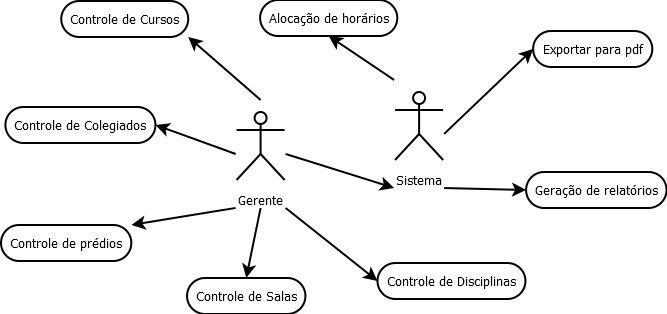
\includegraphics[scale=0.5]{diagramaCasoUso.png}
   		\\ \textbf{\footnotesize Fonte: Autor}
	\end{figure}


\subsubsecao{Diagrama de Atividade: Alocação}
	
	Descrever a rotina de atividades da alocação do sistema
	

\subsubsecao{Diagrama de Classe das controllers}
		
	Achar alguma referencia de diagrama de classe.

	Imagem do diagrama de classe das controllers

\subsubsecao{Diagrama de Classe das models}
	
	Imagem do diagrama de classe das models

\subsubsecao{Diagrama de Classe das views}
	
	Imagem do diagrama de classe das views

\subsubsecao{Modelagem de Dados}

	Achar alguma referencia de modelagem de dados

	Inserir imagem do modelo

		\begin{figure}[!htb]
   		\caption[Modelagem Banco de Dados]{Modelagem Banco de Dados}
   		\label{fig:figura3}
   		\centering
   		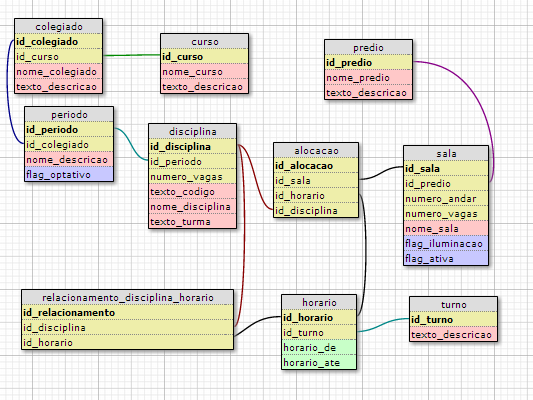
\includegraphics{modelagemBanco.png}
   		\\ \textbf{\footnotesize Fonte: Autor}
	\end{figure}

\subsecao{Interface}

	Achar alguma referencia sobre interface
	
	Twitter bootstrap.\par

\subsecao{Funcionalidades}

	O sistema consiste nas seguintes funcionalidades.

	1. Controle de cursos \par
	2. Controle de colegiados\par
	3. Controle de disciplinas\par
	4. Controle de salas\par
	5. Controle de prédios\par
	6. Alocação de horários\par
	7. Geração de relatórios\par
	8. Exportar para pdf\par



\subsecao{Dados de Entrada}

	Como serão inseriadas as informações, e quais são os dados de entrada

	Informados pelo gerente.

\subsecao{Alocação}

	Processa os dados de alocação

\subsecao{Relatórios}

	Geração dos relatorios determinados na analise do sistema, todos os relatorios podem ser exportados para pdf

\subsecao{Considerações Finais do Capítulo}

Considerações finais do capitulo